\documentclass[11pt]{article}

\usepackage[margin=1in]{geometry}
\usepackage{amsmath}
\usepackage{array}
\usepackage{booktabs}
\usepackage{graphicx}
\usepackage{hyperref}
\usepackage{natbib}
\usepackage{placeins}

\graphicspath{{../results/figures/}}

\title{Algorithmic Complexity Analysis of Ensemble Methods for Real-Time Malaria Outbreak Prediction in Uganda}
\author{Ayiko Andrew}
\date{March 2026}

\begin{document}
\maketitle

\begin{abstract}
Machine learning models for malaria early warning are often judged by predictive accuracy, but deployment in resource-limited public health settings also depends on training cost, inference latency, and memory footprint. This paper argues that the best ensemble method for CPU-only malaria surveillance is regime-dependent: Random Forest is competitive for very small ensembles, while LightGBM becomes the stronger computational choice as ensemble size increases. We compare both methods using engineered Uganda malaria surveillance features derived from public aggregate WHO malaria indicators, regional admissions records, and processed health-sector indicators, yielding 129 observations and 19 model features for high-burden classification. The analysis combines theoretical complexity bounds for training, inference, and storage with empirical profiling over ensemble size $k$, feature dimension $d$, sample size $n$, tree depth $h$, and potential CPU parallelism $p$. In the small-ensemble setting ($k=10$), sequential Random Forest profiling has lower training overhead (267.6 ms) than LightGBM (672.4 ms), reflecting low setup cost for small ensembles. By $k=100$ at depth 5, the crossover reverses: LightGBM reduces training time from 3865.3 ms to 898.0 ms and inference time from 26.35 ms to 9.10 ms. Both methods remain well within sub-second prediction latency and the six-hour daily retraining constraint, but their trade-offs differ. The findings support choosing Random Forest for low-overhead, small-ensemble deployments and LightGBM for larger ensembles where histogram-based training provides better scaling on standard CPU hardware.
\end{abstract}

\section{Introduction}
Malaria remains a major public health burden in Uganda, where timely surveillance and early warning can support district-level planning, commodity allocation, and outbreak response. Ensemble machine learning methods are attractive for this task because they can model nonlinear relationships among incidence, mortality, admissions, intervention coverage, temporal lag features, and regional effects. However, model accuracy alone is not sufficient for deployment. In resource-limited settings, outbreak prediction systems must run on standard CPU hardware, often without GPU acceleration or large memory budgets.

This paper studies the computational feasibility of ensemble methods for malaria outbreak prediction. The central research question is: what are the theoretical and empirical time and space complexity bounds of Random Forest and LightGBM for real-time outbreak prediction, and which configurations meet resource-limited deployment constraints on standard CPU hardware? We focus on three operational constraints: prediction latency below one second, training time below six hours for daily model updates, and memory usage compatible with ordinary district-level computers.

These thresholds are intended to represent practical decision-support use rather than theoretical limits. Sub-second inference keeps predictions responsive inside an interactive dashboard or routine review workflow, where delays can discourage use by busy health workers. A six-hour training budget allows a model to be refreshed within a daily or overnight reporting cycle after new surveillance data are aggregated. The memory constraint reflects a low-cost CPU deployment assumption: a usable model should not require specialized accelerators or large server-class hardware before it can support district or program-level analysis.

The contribution is threefold. First, we provide a focused complexity derivation for Random Forest and LightGBM in the outbreak prediction setting. Second, we empirically profile training time, inference latency, memory footprint, and predictive performance using engineered Uganda malaria surveillance features. Third, we identify the practical crossover behavior between Random Forest and LightGBM across ensemble sizes. Although the empirical case study is Uganda-specific, the complexity argument is broader: it gives low-resource public health teams a way to choose ensemble methods according to data size, feature dimension, update frequency, and available CPU hardware rather than accuracy alone.

\section{Related Work}
Malaria early-warning research in Africa predates current machine learning pipelines and has long emphasized timely detection, climate sensitivity, and operational response. \citet{thomson2001malaria} framed Malaria Early Warning Systems as a public-health need for Africa, while \citet{abeku2004highlands} examined epidemic warning and detection in African highland settings. Subsequent work developed and validated rainfall, sea-surface-temperature, remote-sensing, and ecosystem-based malaria prediction models in Botswana, Ethiopia, and East Africa \citep{thomson2005botswana,midekisa2012remote,githeko2014eastafrica}. Uganda is also part of this operational history: \citet{mueller2009costs} studied the costs of early detection systems for epidemic malaria in highland areas of Kenya and Uganda. This literature motivates prediction as a surveillance tool, but its primary evaluation focus is epidemiological validity, signal detection, or program cost rather than the computational profile of candidate machine learning models.

The broader outbreak forecasting literature similarly emphasizes predictive performance and public-health signal quality. Reviews of infectious-disease forecasting document many modeling strategies and evaluation choices, but deployment metrics such as wall-clock training time, per-prediction latency, and memory footprint are not usually treated as primary outcomes \citep{nsoesie2014forecasting}. Modern machine learning studies for outbreak prediction, including data-integration and multitask learning approaches, extend the modeling toolkit but generally foreground prediction accuracy, feature integration, or event detection rather than CPU-only feasibility \citep{bardak2017outbreak}. For resource-limited health systems, that omission matters: a model that is accurate but slow to retrain, difficult to run locally, or memory-intensive may be impractical for routine surveillance workflows.

Algorithmic work provides the complexity tools needed to close this deployment gap. Random Forest was introduced by \citet{breiman2001random} as an ensemble of decision trees trained on bootstrap samples with random feature selection. Its strength for CPU deployment comes from the independence of individual trees, which allows near-trivial parallelism across cores. \citet{louppe2014understanding} provides a detailed theoretical account of Random Forest training and inference complexity, including the role of sorting during split selection. Gradient boosting builds trees sequentially, fitting each new tree to residual structure left by previous trees \citep{friedman2001greedy}. XGBoost introduced scalable tree boosting with regularization and cache-aware computation \citep{chen2016xgboost}. LightGBM further improves computational efficiency through histogram-based split finding, leaf-wise tree growth, Gradient-based One-Side Sampling, and Exclusive Feature Bundling \citep{ke2017lightgbm}. These optimizations reduce the dominant split-search cost from exact sorting toward linear scans over binned features.

The missing link is a study that connects these two bodies of work: malaria early-warning models on one side and algorithmic complexity analysis on the other. To our knowledge, prior malaria prediction studies in sub-Saharan Africa have not profiled Random Forest and LightGBM training time, inference latency, and memory footprint under CPU-only constraints as the central research object. This paper addresses that gap by treating computational complexity not as an implementation detail, but as a deployment criterion for real-time public health decision support.

\section{Data and Feature Engineering}
The empirical analysis uses public aggregate malaria surveillance data for Uganda. The raw malaria indicator file is a World Health Organization Global Health Observatory data product accessed through the Humanitarian Data Exchange Uganda dataset \citep{ugandaWHOData}. It contains national Uganda indicators from 2000 to 2024, including estimated malaria mortality, estimated incidence, total malaria cases, suspected cases, microscopy examinations, and microscopy-positive cases. The engineered model matrix used for the profiling experiments is built from cleaned regional malaria admission reports from the Uganda Health Data Observatory \citep{MoHUganda2026} and supplementary processed health-sector indicators. After cleaning and lag construction, the final matrix covers 2020--2024, contains 129 region-year observations from 14 Uganda regions, and includes 19 model features. The regions represented are Acholi, Ankole, Buganda, Bugisu, Bukedi, Bunyoro, Busoga, Kampala, Karamoja, Kigezi, Lango, Teso, Tooro, and West Nile.

The feature engineering pipeline is admissions-centered because the final modeling table is organized at the regional admission-report level. Table~\ref{tab:feature-engineering} summarizes the exact feature groups. Lag features use the previous one and two reporting periods for each region. Rolling features use two- and three-period windows to capture recent local admission levels, volatility, and peaks. Change features capture absolute and proportional movement from the previous observation. Regional summary features encode each region and summarize its historical admission distribution. National-context features compare each region-year observation with the corresponding national admission distribution for that year. The binary target, \texttt{outbreak}, is a high-burden indicator equal to one when admissions exceed the engineered threshold of 65 admissions; it should therefore be interpreted as high-burden or early-warning classification rather than an official outbreak declaration.

\begin{table}[ht]
\centering
\caption{Engineered feature groups used in the complexity experiments.}
\label{tab:feature-engineering}
\renewcommand{\arraystretch}{1.18}
\resizebox{\textwidth}{!}{%
\begin{tabular}{>{\raggedright\arraybackslash}p{0.20\textwidth} >{\raggedright\arraybackslash}p{0.36\textwidth} >{\raggedright\arraybackslash}p{0.36\textwidth}}
\toprule
Group & Features & Construction \\
\midrule
Lagged admissions & \texttt{admissions\_lag\_1}, \texttt{admissions\_lag\_2} & Previous one and two regional reporting periods \\
Rolling level and volatility & \texttt{admissions\_roll\_mean\_2}, \texttt{admissions\_roll\_std\_2}, \texttt{admissions\_roll\_max\_2} & Mean, standard deviation, and maximum over two periods \\
Rolling level and volatility & \texttt{admissions\_roll\_mean\_3}, \texttt{admissions\_roll\_std\_3}, \texttt{admissions\_roll\_max\_3} & Mean, standard deviation, and maximum over three periods \\
Change features & \texttt{admissions\_change}, \texttt{admissions\_pct\_change} & Absolute and proportional change from previous observation \\
Regional context & \texttt{region\_encoded}, \texttt{region\_mean}, \texttt{region\_std}, \texttt{region\_min}, \texttt{region\_max} & Region code and historical regional admission summaries \\
National context & \texttt{national\_mean}, \texttt{national\_std}, \texttt{relative\_to\_national}, \texttt{deviation\_from\_national} & Annual national admission summaries and regional deviation from them \\
\bottomrule
\end{tabular}%
}
\renewcommand{\arraystretch}{1.0}
\end{table}

For the complexity experiments, the 129 observations are split into 103 training observations and 26 test observations using a stratified 80/20 random split. This choice preserves both classes in a small dataset and gives a fixed held-out batch for measuring inference latency across model configurations. It is appropriate for the computational question in this paper because the primary outcomes are training time, inference time, and memory use under identical data dimensions. It is not presented as a definitive prospective surveillance validation design. Because the data have temporal structure, a future operational accuracy study should use a time-aware split or rolling-origin evaluation so that later observations cannot inform earlier predictions. Accordingly, predictive accuracy in this paper is treated as a feasibility check, while the central evidence is the comparative complexity profile.

All data used in the analysis are public, aggregate, and non-identifiable. The study does not use individual patient records. Local institutional requirements should still be confirmed for any operational deployment, especially if future versions integrate facility-level or patient-level data. The feature engineering pipeline, profiling scripts, processed tables, and manuscript materials are available at \url{https://github.com/Ayikoandrew/ensemble-outbreak-complexity}.

\section{Methods}
\subsection{Models}
We compare two ensemble methods. Random Forest is implemented as a bagged ensemble of decision trees with independent tree construction; this structure supports CPU parallelism over trees, although the reported runs use sequential tree construction. LightGBM is implemented as histogram-based gradient boosting, where trees are added sequentially and split search is accelerated using binned feature histograms. Logistic regression and a single decision tree are included as baseline references for computational scale, not as models that the ensembles must outperform on this small dataset.

This distinction is important because the engineered classification task is highly separable: the baseline models already achieve very high held-out accuracy in the profiling split reported later in the paper. The experiment is therefore designed as a computational profiling study rather than a claim that ensembles are needed for predictive superiority on these 129 observations. Accuracy is reported for completeness and to verify that models are learning the target, but the primary outcomes are wall-clock training time, batch inference latency, and memory footprint under fixed data dimensions.

The main ensemble sweep varies the number of estimators and maximum tree depth. Random Forest configurations include $k \in \{10,50,100,200\}$ and depths 5, 10, and 15. LightGBM configurations include $k \in \{10,50,100,200\}$, depths 5, 10, and 15, and leaf counts matched to the depth regimes. Each configuration is profiled on the same train/test split so that measured differences reflect algorithmic and implementation costs rather than changing data size or feature composition. The reported Random Forest timings use scikit-learn's \texttt{n\_jobs=1}, so they measure sequential tree construction rather than tree-level parallel training. LightGBM is run on CPU with column-wise histogram construction; its internal threading is left to the library default. The $p$ terms in the theoretical analysis therefore describe potential CPU parallelism for deployment, while the empirical RF timings should be interpreted as the $p=1$ case. The primary profiling table reports single-run measurements from the notebook; a 10-repeat diagnostic on the depth-5 $k\in\{10,50,100\}$ configurations found coefficient-of-variation values of 7.5--12.7\% for Random Forest and 53.8--79.5\% for LightGBM, indicating that the crossover estimate should be read as approximate rather than exact. The higher LightGBM variance is expected for short small-data fits because Python-level initialization, histogram setup, and library scheduling overhead can form a large share of total runtime, so small absolute timing fluctuations translate into large relative variation.

\subsection{Deployment Constraints}
The deployment scenario assumes standard CPU hardware with no GPU acceleration. Table~\ref{tab:deployment-constraints} summarizes the operational thresholds used to judge computational feasibility. These thresholds are intentionally conservative relative to the dataset scale in this study, but they make the profiling exercise interpretable as a deployment screen rather than a purely academic timing benchmark.

\begin{table}[ht]
\centering
\caption{Deployment constraints used for computational feasibility screening.}
\label{tab:deployment-constraints}
\begin{tabular}{>{\raggedright\arraybackslash}p{0.20\textwidth} >{\raggedright\arraybackslash}p{0.22\textwidth} >{\raggedright\arraybackslash}p{0.48\textwidth}}
\toprule
Constraint & Threshold & Operational rationale \\
\midrule
Inference latency & $<1$ second per prediction & Supports responsive dashboards and routine case-review workflows \\
Training time & $<6$ hours per update & Allows daily or overnight model refresh after surveillance data aggregation \\
Memory footprint & $<16$ GB RAM & Keeps the model compatible with low-cost CPU machines rather than server-class hardware \\
Hardware & CPU only & Tests feasibility without GPUs or specialized accelerators \\
\bottomrule
\end{tabular}
\end{table}

\section{Complexity Analysis}
Let $n$ denote the number of training samples, $d$ the number of features, $k$ the number of trees, $h$ the average tree depth, $b$ the number of LightGBM histogram bins, and $p$ the number of usable CPU cores. The base of the logarithm is asymptotically irrelevant and is absorbed into the constants; for the numerical crossover calculation below, $\log_2 n$ is used explicitly.

\subsection{Random Forest}
A decision tree using exact split search sorts feature values or otherwise evaluates ordered split candidates. For a balanced tree, the dominant training cost is commonly expressed as
\begin{equation}
T_{\mathrm{tree}} = O(n d \log n).
\end{equation}
This bound should be read as the standard exact-split abstraction rather than a literal description of every low-level operation in the library implementation. Scikit-learn's tree routines are implemented in optimized compiled code and avoid Python-level sorting at each node; those implementation choices affect constants, while the $n d \log n$ term captures the cost of ordered split search used for the theoretical comparison.
For $k$ trees, sequential Random Forest training is
\begin{equation}
T_{\mathrm{RF}} = O(k n d \log n).
\end{equation}
Because trees are independent, training can be parallelized across $p$ CPU cores in implementations that enable tree-level parallelism, giving the practical bound
\begin{equation}
T_{\mathrm{RF,parallel}} = O\left(\frac{k n d \log n}{p}\right).
\end{equation}
The empirical results in this paper, however, use \texttt{n\_jobs=1} for scikit-learn Random Forest, so the measured RF timings correspond to the sequential case $p=1$. Equation~(3) is retained to show how the same model could scale under a parallel deployment configuration.
For inference, each tree follows one path from root to leaf, so per-sample inference is
\begin{equation}
I_{\mathrm{RF}} = O(kh).
\end{equation}
Model storage scales with the number of trees and tree nodes, approximately
\begin{equation}
S_{\mathrm{RF}} = O(k2^h)
\end{equation}
for depth-limited balanced trees. This upper bound remains tractable at the depths profiled here. For example, a full binary tree of depth 15 has $2^{15}=32{,}768$ possible leaf-scale units under this simplified bound; even 200 such trees imply about $6.55\times 10^6$ units before implementation-specific compression and early stopping from pure or empty leaves.

\subsection{LightGBM}
LightGBM replaces exact split sorting with histogram-based split finding. Continuous features are binned into $b$ bins, where $b$ is typically treated as a constant. Histogram construction and scanning reduce the per-tree split-search burden toward linear dependence on $n$ and $d$, yielding
\begin{equation}
T_{\mathrm{LGB}} = O(knd).
\end{equation}
Boosting is sequential across trees, so LightGBM does not parallelize over $k$ in the same way Random Forest does. It can, however, exploit CPU parallelism within histogram construction and feature scans. Per-sample inference traverses one path in each boosted tree:
\begin{equation}
I_{\mathrm{LGB}} = O(kh).
\end{equation}
Space complexity includes tree storage plus histogram and gradient buffers. A simplified model-storage bound is again $O(k2^h)$, while training memory has additional histogram-dependent overhead.

\subsection{Expected Crossover}
Ignoring constant factors, LightGBM is faster than potentially parallel Random Forest when
\begin{equation}
C_{\mathrm{LGB}} knd < C_{\mathrm{RF}} \frac{knd\log n}{p},
\end{equation}
where $C_{\mathrm{LGB}}$ and $C_{\mathrm{RF}}$ represent implementation and hardware constants. After cancellation, the crossover depends on $\log n$, CPU parallelism, and constant overheads:
\begin{equation}
p < \frac{C_{\mathrm{RF}}}{C_{\mathrm{LGB}}}\log n.
\end{equation}
For small $n$ and small $k$, LightGBM's histogram overhead can dominate. As $k$ grows, LightGBM's lower per-tree training cost can outweigh that overhead. If Random Forest parallelism is enabled, the crossover can shift because effective $p$ reduces RF training time; that shift is not measured in the reported \texttt{n\_jobs=1} experiments. Setting $p=1$ recovers the sequential Random Forest case actually tested, while the $p$-dependent form is retained to show how the crossover would shift when tree-level parallelism is enabled.

The profiling data provide an empirical check on this crossover model for the sequential RF setting actually tested. Using base-2 logarithms for the numeric calculation, rearranging Equation~(9) gives
\begin{equation}
\frac{C_{\mathrm{RF}}}{C_{\mathrm{LGB}}} \approx \frac{T_{\mathrm{RF}}}{T_{\mathrm{LGB}}}\frac{p}{\log_2 n}.
\end{equation}
With \texttt{n\_jobs=1}, $p=1$ for the Random Forest measurements. In the depth-5 sweep, $n=103$ training samples and $\log_2 n \approx 6.69$. At $k=10$, the measured time ratio is $267.6/672.4=0.40$, so the implied $C_{\mathrm{RF}}/C_{\mathrm{LGB}}$ is approximately $0.060$ and Random Forest is faster. At $k=50$, the measured ratio rises to $1217.7/773.2=1.58$, implying $C_{\mathrm{RF}}/C_{\mathrm{LGB}} \approx 0.236$; because the right-hand side of Equation~(9) is then greater than the measured $p=1$, LightGBM becomes faster. By $k=100$, the ratio is $3865.3/898.0=4.30$, implying $C_{\mathrm{RF}}/C_{\mathrm{LGB}} \approx 0.644$. These constants are not universal, and a rerun with \texttt{n\_jobs=2} could move the observed crossover. The timing-variance diagnostic reinforces that the value should be interpreted as a local crossover region, not a precise universal threshold. The empirical pattern still validates the framework for the tested configuration: the practical crossover is governed by asymptotic split-search cost, implementation overhead, measurement variance, and the degree of parallelism actually enabled.

\section{Results}
\subsection{Baseline Model Comparison}
Table~\ref{tab:complexity-summary} summarizes the main publication-ready comparison. All models meet the sub-second inference requirement by a wide margin. The held-out test batch contains 26 observations, including 6 positive high-burden cases and 20 negative cases, so accuracy alone is not a sufficient evaluation metric: a trivial all-negative classifier would already reach 0.769 accuracy. For that reason, the table reports positive-class precision, recall, F1, and AUC in addition to accuracy. These metrics confirm that the task is highly separable in this split; they do not establish that ensembles are epidemiologically superior to the simpler baselines.

\begin{table}[ht]
\centering
\caption{Computational and predictive profiling summary for malaria outbreak prediction.}
\label{tab:complexity-summary}
\resizebox{\textwidth}{!}{%
\begin{tabular}{l l l r r r r r r r r}
\toprule
Model & Training & Inference & Train ms & Infer ms & Memory MB & Acc. & Prec.+ & Rec.+ & F1+ & AUC \\
\midrule
Logistic Regression & $O(ndi)$ & $O(d)$ & 302.1 & 1.08 & 0.046 & 1.000 & 1.000 & 1.000 & 1.000 & 1.000 \\
Decision Tree & $O(nd\log n)$ & $O(h)$ & 53.2 & 1.00 & 0.027 & 0.962 & 1.000 & 0.833 & 0.909 & 0.917 \\
Random Forest ($k=100$) & $O(knd\log n)$ & $O(kh)$ & 3865.3 & 26.35 & 0.113 & 1.000 & 1.000 & 1.000 & 1.000 & 1.000 \\
LightGBM ($k=100$) & $O(knd)$ & $O(kh)$ & 898.0 & 9.10 & 1.096 & 0.962 & 1.000 & 0.833 & 0.909 & 0.846 \\
\bottomrule
\end{tabular}%
}
\end{table}

At $k=100$ and depth 5, LightGBM trains approximately 4.3 times faster than Random Forest and performs inference approximately 2.9 times faster. Random Forest uses less measured memory, while LightGBM's memory footprint is higher because of histogram and boosting data structures. Both memory footprints are small in absolute terms.

\subsection{Ensemble Scaling}
The ensemble sweep reveals the practical crossover. At $k=10$ and depth 5, sequential Random Forest trains in 267.6 ms compared with 672.4 ms for LightGBM. This supports the hypothesis that RF can be preferable for very small ensembles on CPU because its setup overhead is low and LightGBM pays fixed histogram-construction costs. However, because this small-$k$ LightGBM fit is especially sensitive to initialization and scheduling overhead, the $k=10$ comparison should carry less inferential weight than the larger-ensemble comparisons. At $k=50$ and depth 5, the pattern reverses: Random Forest trains in 1217.7 ms while LightGBM trains in 773.2 ms. At $k=100$ and depth 5, the gap widens further, with Random Forest at 3865.3 ms and LightGBM at 898.0 ms.

The depth sweep shows that LightGBM's advantage is not limited to shallow trees. At $k=100$, Random Forest training time is 3865.3 ms at depth 5, 2455.0 ms at depth 10, and 4061.0 ms at depth 15. LightGBM is faster in all three settings: 898.0 ms, 105.6 ms, and 233.7 ms, respectively. The pattern is not strictly monotonic because maximum depth is an upper bound rather than the realized depth of every tree, and the dataset is small enough that pure or low-sample leaves can terminate growth early. LightGBM's leaf-wise growth makes this especially plausible: the algorithm expands the leaf with the largest loss reduction rather than filling every level, so allowing a larger maximum depth does not force substantially more split evaluations when few leaves remain useful. Still, the deeper configurations strengthen rather than weaken the empirical conclusion: LightGBM's histogram-based training remains cheaper than Random Forest's exact-split ensemble construction across the profiled depth range.

These results validate the crossover model derived in Section~5.3. In the depth-5 sweep, the implied constant ratios $C_{\mathrm{RF}}/C_{\mathrm{LGB}}$ rise from 0.060 at $k=10$ to 0.236 at $k=50$ and 0.644 at $k=100$. The increase is not interpreted as a universal property of the algorithms; it shows that, on this CPU-only configuration, fixed LightGBM overhead dominates at very small $k$ while Random Forest's exact-split ensemble cost dominates as $k$ grows. Thus the empirical profiling results provide direct support for the crossover mechanism rather than only a descriptive timing comparison.

\begin{figure}[!htbp]
\centering
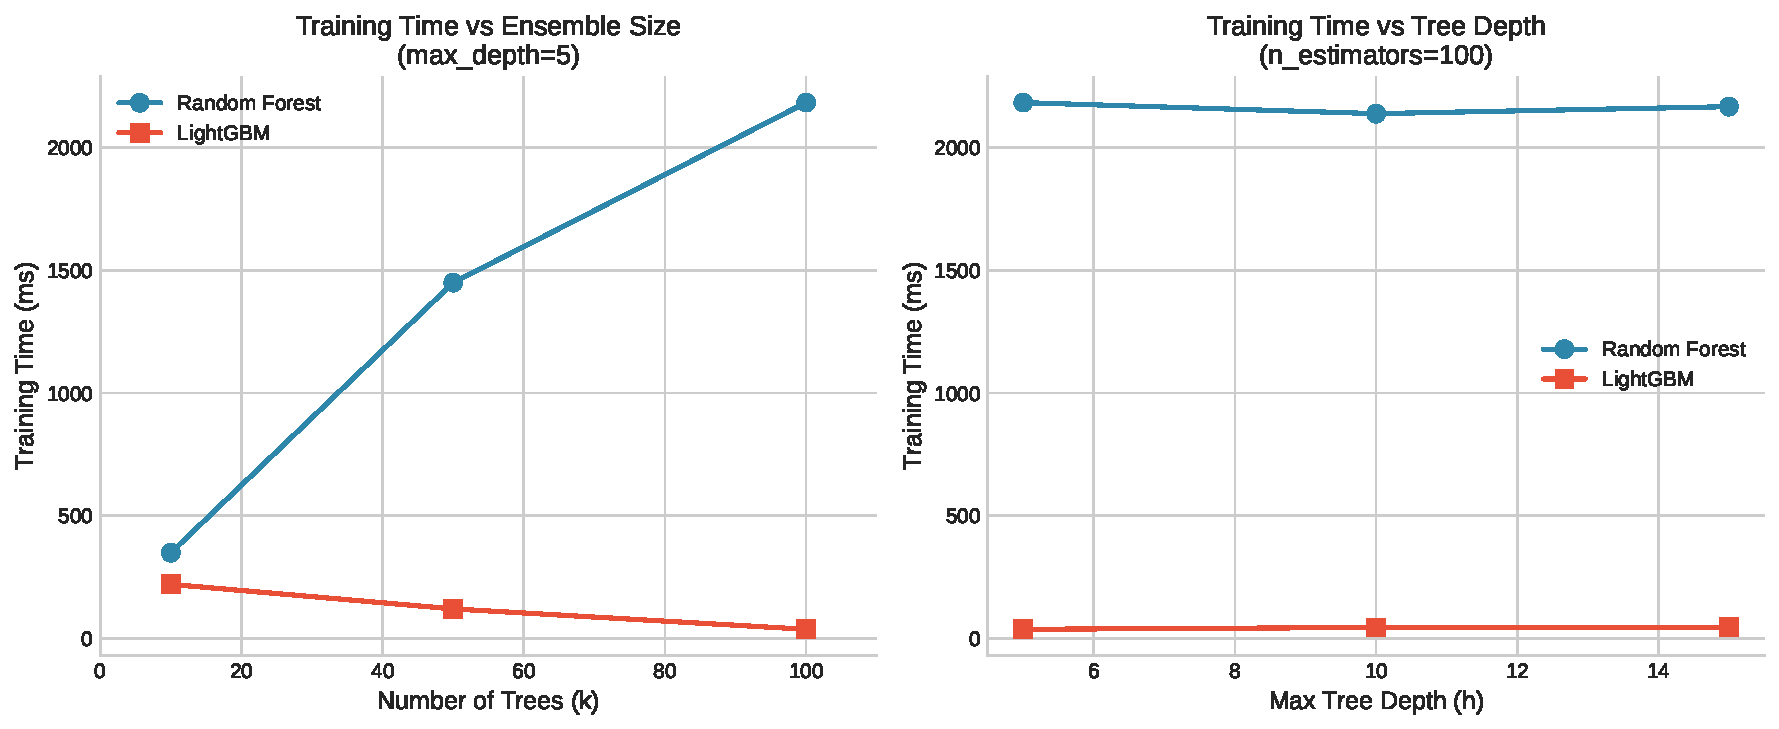
\includegraphics[width=0.88\textwidth]{fig1_training_time_scaling.pdf}
\caption{Training time scaling across Random Forest and LightGBM configurations.}
\label{fig:training-scaling}
\end{figure}

\begin{figure}[!htbp]
\centering
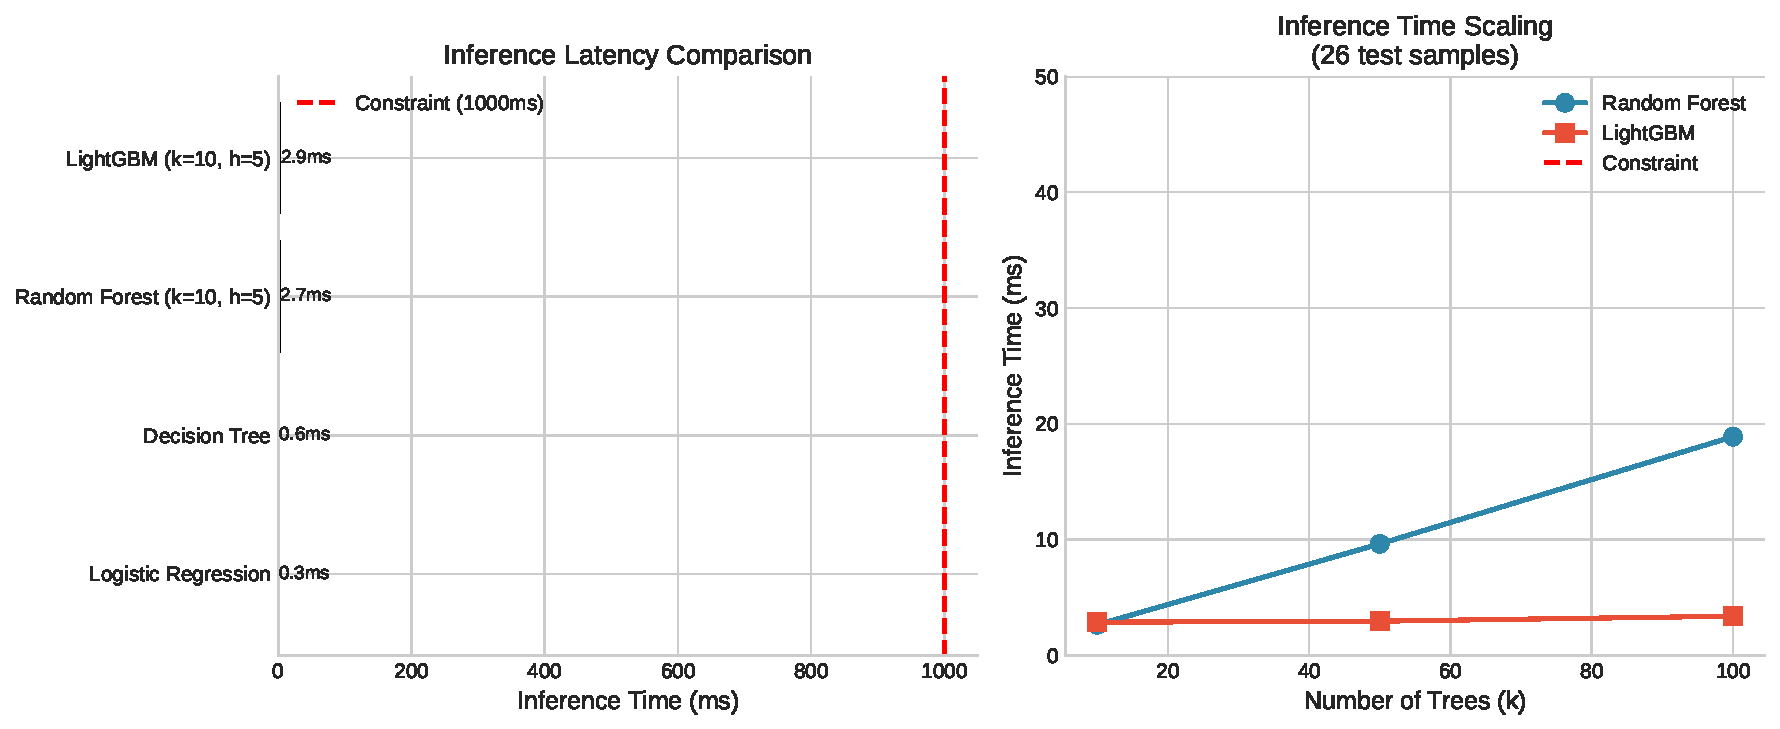
\includegraphics[width=0.88\textwidth]{fig2_inference_latency.pdf}
\caption{Inference latency across profiled configurations. All measured configurations are below the one-second real-time threshold.}
\label{fig:inference-latency}
\end{figure}

\FloatBarrier

\subsection{Memory and Accuracy Trade-Offs}
Random Forest consistently uses less measured memory than LightGBM in the profiling tables. For example, at $k=100$ and depth 5, Random Forest uses 0.113 MB while LightGBM uses 1.096 MB. This is a roughly tenfold difference, but both are far below the memory budgets of ordinary 8--16 GB CPU machines. Mechanistically, LightGBM's training memory includes more than the final tree structures: it also maintains compact binned feature representations, gradient and Hessian buffers of size $O(n)$, and feature-bin histograms that scale with the number of features, bins, and active leaves. Those auxiliary buffers explain why LightGBM can train faster while using more memory in this small-data setting.

\begin{figure}[!htbp]
\centering
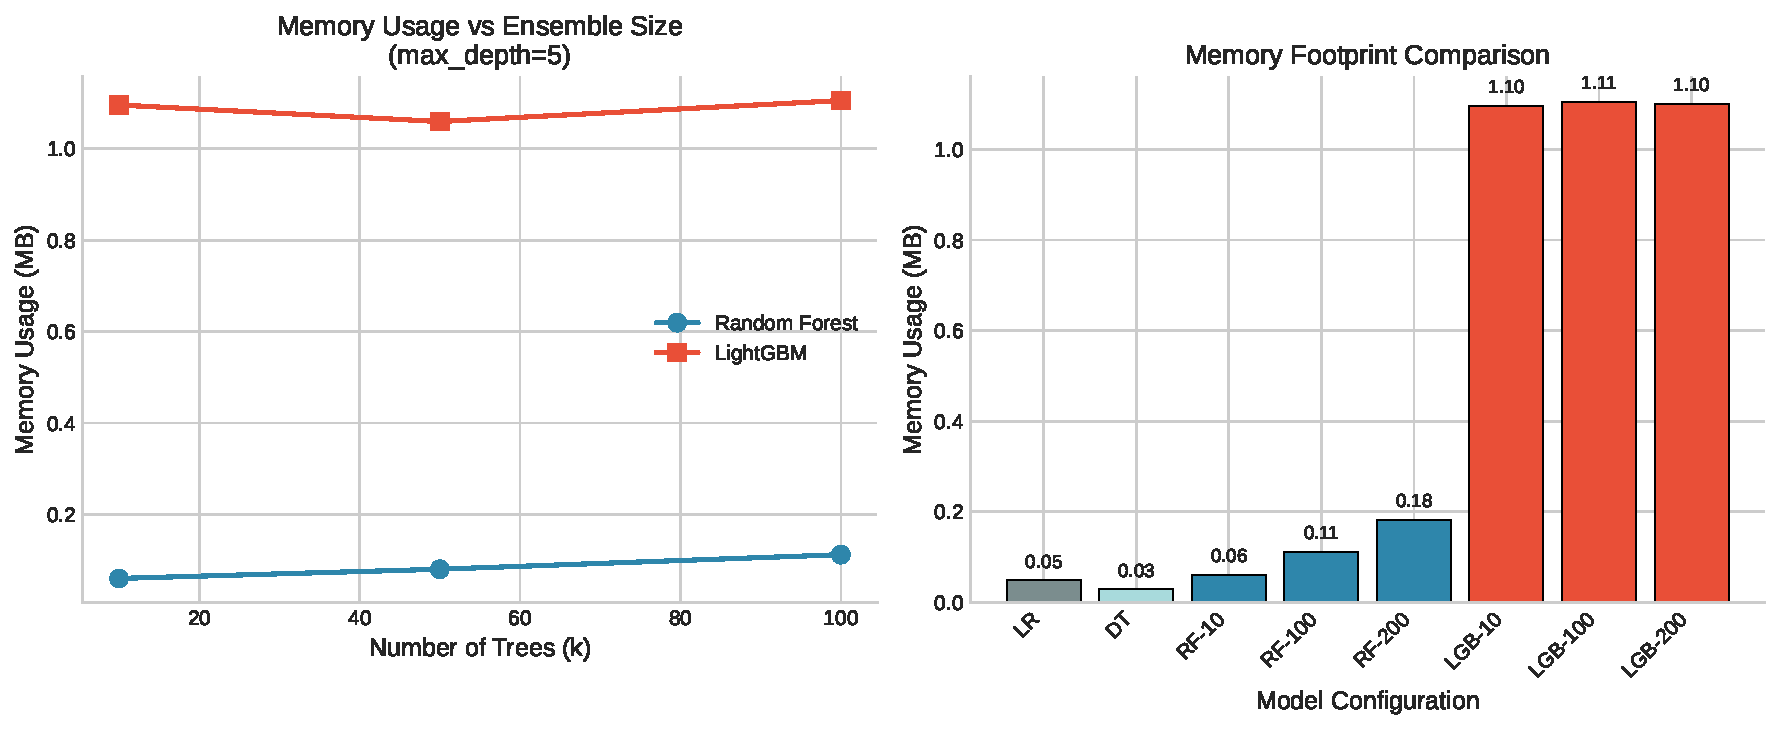
\includegraphics[width=0.88\textwidth]{fig3_memory_footprint.pdf}
\caption{Measured memory footprint for profiled models. LightGBM uses more memory but remains within practical CPU-only deployment limits.}
\label{fig:memory}
\end{figure}

Predictive metrics are high for all models, which reinforces the methodological framing of this paper. Logistic regression and Random Forest both reach perfect held-out accuracy and AUC in the profiling split, while the decision tree and LightGBM each miss one of the six positive cases, giving recall 0.833 and F1 0.909. These differences should be interpreted cautiously because the dataset is small and the target is highly separable. For deployment decisions based on this experiment, the central result is therefore computational: the models are accurate enough to make profiling meaningful, but the evidence distinguishing Random Forest from LightGBM is training time, inference latency, and memory use rather than a robust accuracy gap.

In Figure~\ref{fig:accuracy-cost}, the y-axis is held-out accuracy for all plotted models. The dashed horizontal line marks a 0.85 target threshold used as a conservative feasibility floor for this computational screening exercise, not an AUC value or a validated epidemiological decision threshold. Bubble area scales with ensemble size $k$, so larger bubbles represent computationally heavier configurations.

\begin{figure}[!htbp]
\centering
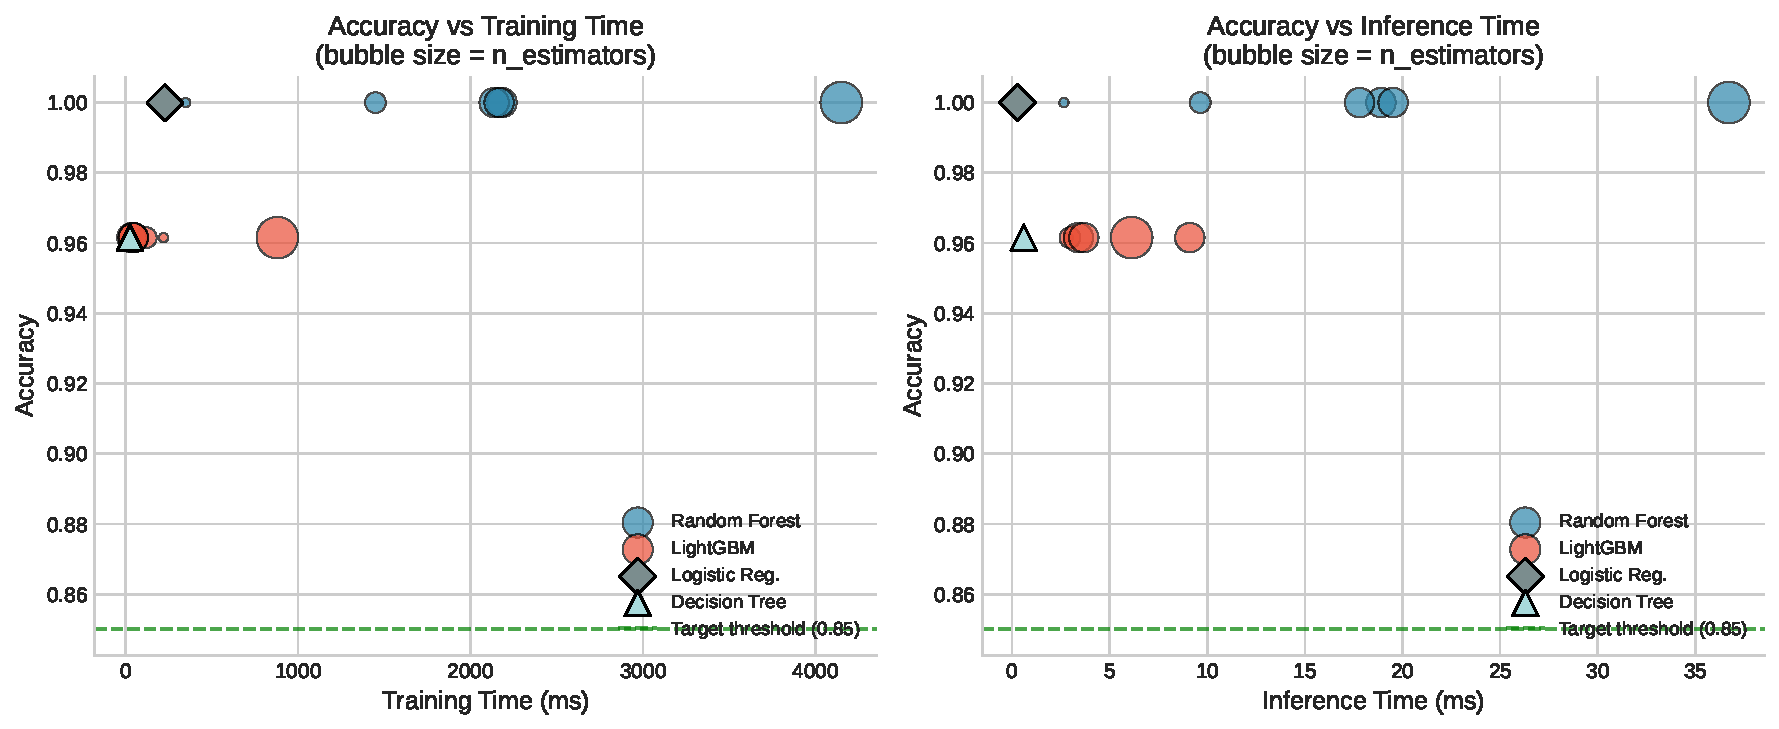
\includegraphics[width=0.88\textwidth]{fig4_accuracy_vs_cost.pdf}
\caption{Predictive feasibility versus computational cost for baseline and ensemble models. The dashed line marks a conservative 0.85 feasibility floor on the accuracy axis.}
\label{fig:accuracy-cost}
\end{figure}

\FloatBarrier

\section{Discussion}
The results show that asymptotic complexity alone does not determine the best model in the small-data regime. LightGBM has the stronger theoretical training bound, $O(knd)$, but sequential Random Forest can be faster at small $k$ because it has low setup overhead. Random Forest also has a potential deployment advantage when tree-level parallelism is enabled, but the reported profiling runs did not use that option. This matters for outbreak prediction systems trained on limited surveillance histories, where $n$ may be closer to hundreds than millions.

The crossover observed in the profiling sweep is practically important. Linear interpolation between the measured $k=10$ and $k=50$ depth-5 runs places the training-time crossover at approximately $k=29$ for the sequential \texttt{n\_jobs=1} Random Forest setting. This estimate should not be treated as a universal constant, because it depends on hardware, implementation, depth, data size, enabled threading, and timing variance; repeated runs could plausibly shift the local threshold toward smaller or larger $k$. The high relative variance in short LightGBM fits reinforces this interpretation, because overhead-dominated small-$k$ timings can narrow or widen the apparent gap even when the asymptotic trend is unchanged. The practical claim is therefore weaker at $k=10$ than at $k=100$: the small-ensemble RF advantage is plausible but noisy, whereas the larger-ensemble LightGBM advantage is supported by a much wider separation in measured training time. For CPU-only deployments using roughly fewer than 25--30 trees, Random Forest is likely to be competitive or faster because of low setup overhead. Once the model requires larger ensembles, LightGBM's histogram-based optimization dominates in the tested configuration: at $k=50$, LightGBM is already faster than Random Forest; at $k=100$, it is substantially faster in both training and inference. Therefore, for models requiring larger ensembles to achieve stable performance, LightGBM provides the better computational trade-off unless Random Forest is rerun with sufficient tree-level parallelism to shift the crossover.

The memory result cuts in the other direction. Random Forest has a smaller measured footprint in this study, while LightGBM's additional histogram and boosting structures increase memory usage. In absolute terms, however, the measured values are small enough that memory does not threaten deployment feasibility for either model. The more relevant operational distinction is training and inference time.

Interpretability is a second deployment consideration beyond speed and memory. Random Forest has a practical advantage for routine explanation because global feature importance summaries are familiar, inexpensive to compute, and relatively easy to communicate to public health managers. LightGBM can also be explained, especially with SHAP-style attribution methods, but those explanations add computational and workflow overhead and may require more technical support. In a district or program setting where users must justify why a region was flagged as high-burden, the final model choice should therefore consider explanation needs alongside runtime. A small Random Forest may be preferable when transparency and local explanation are the dominant requirements; LightGBM is more compelling when larger ensembles are needed and the team can support attribution tooling.

The perfect or near-perfect predictive values also require caution. High scores on a small split can indicate strong separability, leakage, or overfitting. This paper therefore treats predictive performance as a feasibility check rather than a final epidemiological claim. Because all models perform well on the current split, complexity and deployment properties become the deciding axes for model selection. Future work should validate performance under time-aware cross-validation and external temporal holdout periods.

\section{Limitations}
This study has six main limitations. First, the processed real-data profiling table uses only 129 observations, which limits statistical certainty around predictive performance. Second, the empirical sweep varies ensemble size and depth but does not yet provide a full factorial scalability study over large values of $n$. Third, the study does not include external validation: models are trained and tested within the same Uganda surveillance dataset and time period, so generalizability to future reporting periods, finer-grained district data, or other national malaria surveillance systems remains unknown. Fourth, wall-clock measurements are hardware- and implementation-dependent; the theoretical bounds explain trends, but constants determine the exact crossover. The profiling runs reported here were conducted on a CPU-only machine with an Intel Pentium 3558U processor at 1.70 GHz, 2 physical cores, and 7.6 GiB RAM. Random Forest was run with \texttt{n\_jobs=1}, so the empirical results do not measure the speedup available from using both physical cores. A 10-repeat diagnostic on the key depth-5 configurations showed moderate timing variance for Random Forest and high variance for very short LightGBM fits, so the $k\approx29$ crossover should be interpreted as an approximate local finding rather than a stable universal boundary. These specifications make the experiment relevant to low-cost hardware, but they also mean the exact timings should be re-measured on any target deployment machine with explicit threading controls for both Random Forest and LightGBM. Fifth, the outbreak target is derived from aggregate surveillance indicators, so the model should be interpreted as an early-warning classifier rather than a clinical diagnostic system. Sixth, the analysis uses public aggregate data only; operational deployment with facility-level or patient-level data would require additional governance, privacy, and validation review.

\section{Conclusion}
Random Forest and LightGBM both satisfy real-time malaria outbreak prediction constraints on standard CPU hardware in the profiled Uganda surveillance setting. Sequential Random Forest is faster for very small ensembles, training in 267.6 ms versus 672.4 ms for LightGBM at $k=10$. LightGBM becomes faster as ensemble size grows, training in 898.0 ms versus 3865.3 ms for Random Forest at $k=100$, while also reducing inference latency. The practical recommendation is therefore regime-dependent: use Random Forest for small, transparent, low-overhead deployments, especially when interpretability is central; use LightGBM when larger ensembles are needed or when training and inference cost must scale more efficiently. The next step is to repeat the profiling under a temporal holdout design using district-disaggregated Uganda Health Management Information System data, with explicit thread-controlled benchmarks for both models, so that computational feasibility and prospective predictive validity can be evaluated together.

\bibliographystyle{plainnat}
\bibliography{references}

\end{document}
